% Annexe A (après \appendix dans main.tex)
\PFEChapterOpening{Première annexe}
\label{chap:annexe-premiere}

\section{Matrice de Stacey}

\begin{figure}[H]
  \centering
  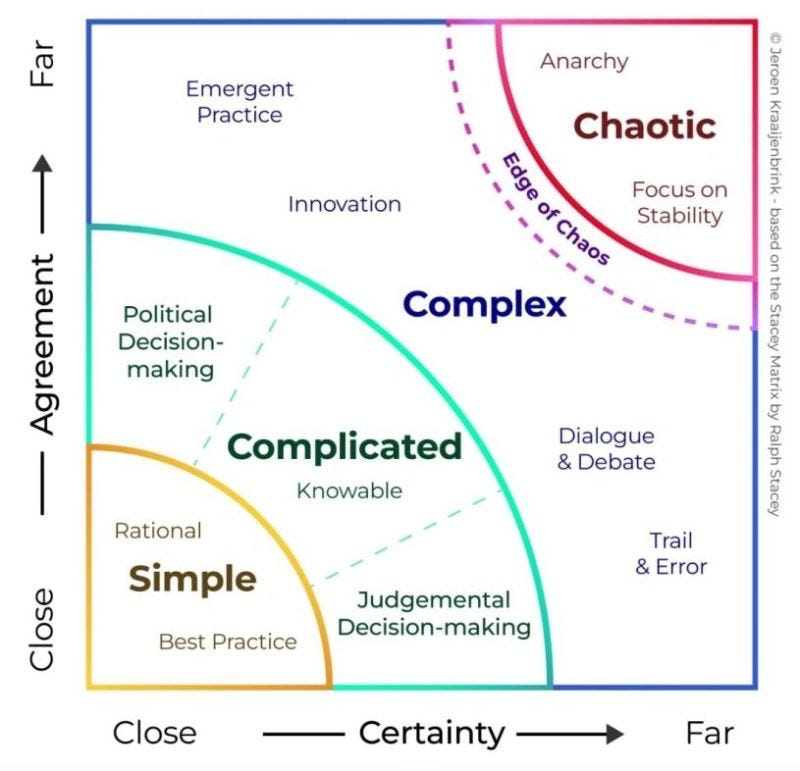
\includegraphics[width=0.75\linewidth]{figures/chapitre-01/matrice-stacey.png}
  \caption{Matrice de Stacey.}\cite{pacheco-stacey-matrix}
  \label{fig:annexe-matrice-stacey}
\end{figure}
